% This file was created by matlab2tikz v0.4.3.
% Copyright (c) 2008--2013, Nico Schlömer <nico.schloemer@gmail.com>
% All rights reserved.
% 
\tikzsetnextfilename{plots/complexTop_eps}
%
% defining custom colors
\definecolor{mycolor1}{rgb}{0,0,0.5625}%
%
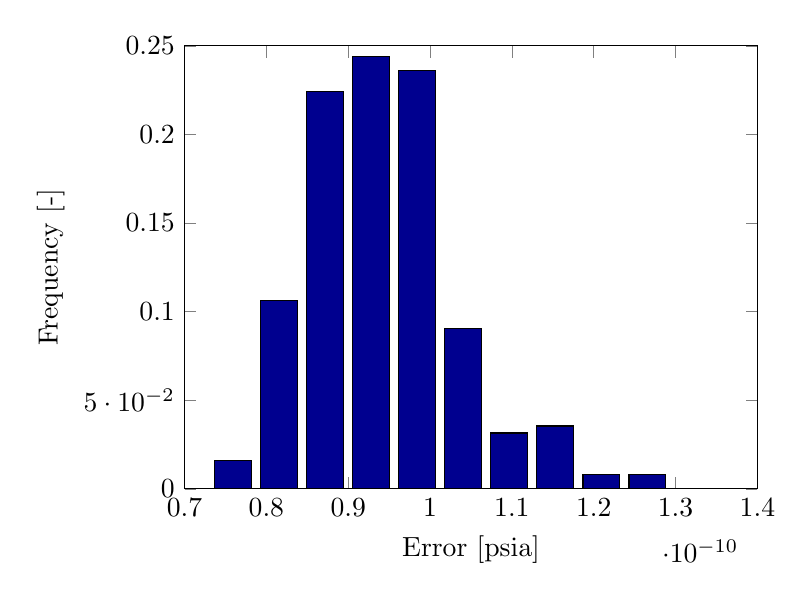
\begin{tikzpicture}

\begin{axis}[%
width=0.6\textwidth,
height=0.464012560662289\textwidth,
area legend,
scale only axis,
xmin=7e-11,
xmax=1.4e-10,
xlabel={Error [psia]},
ymin=0,
ymax=0.25,
ylabel={Frequency [-]}
]
\addplot[ybar,bar width=0.03858856091808\textwidth,draw=black,fill=mycolor1] plot coordinates{(7.59143858886091e-11,0.015748031496063)
(8.15418843558291e-11,0.106299212598425)
(8.71693828230491e-11,0.224409448818898)
(9.27968812902691e-11,0.244094488188976)
(9.84243797574891e-11,0.236220472440945)
(1.04051878224709e-10,0.0905511811023622)
(1.09679376691929e-10,0.031496062992126)
(1.15306875159149e-10,0.0354330708661417)
(1.20934373626369e-10,0.0078740157480315)
(1.26561872093589e-10,0.0078740157480315)};

\addplot [
color=black,
solid,
forget plot
]
table[row sep=crcr]{
7e-11 0\\
1.4e-10 0\\
};
\end{axis}
\end{tikzpicture}%